\section{Pipeline Template}
Our approach integrates data protection and data management into the service pipeline using annotations.
To this aim, we extend the service pipeline in \cref{def:pipeline} with: \emph{i)} functional annotations expressing data manipulations that result from services execution, \emph{ii)} data protection annotations expressing transformations on data to enforce data protection requirements.
These annotations permit to implement an advance data lineage, tracking the entire data lifecycle by monitoring changes arising from functional service execution and data protection requirements.

In the following, we first introduce the annotated service pipeline, pipeline template in Section \ref{sec:templatedefinition}. We then present functional annotations (Section \ref{sec:funcannotation}) and data protection annotations (Section \ref{sec:nonfuncannotation}). We finally provide an example of a pipeline template (Section \ref{sec:example}).


\subsection{Template Definition}\label{sec:templatedefinition}

Given the Pipeline in \cref{def:service_flow}, we use annotations to let the pipeline be aware of the data protection requirements and the functional transformations that will be applied to the data.
Each node is labeled with two mapping functions:
\begin{enumerate*}[label=\roman*)]
  \item a labeling function \myLambda:\V$\rightarrow$\Pset{}, that associates a set of nodes \vi{i}$\in$\V\ to a set of policies $p_i\in$\Pset{}. and
  \item a labeling function \myGamma:\V$\rightarrow$\F{}. that associates a set of nodes \vi{i}$\in$\V\ to a set of data transformation functions $F_i\in\F{}$.

\end{enumerate*}
The policies will be intended to guide the enforcement of data protection while the data transformation function will characterize the functional aspect of each node.

The template is formally defined as follows and and example is depicted in \cref{fig:service_composition_template}.

\begin{definition}[Template] \label{def:template}
  Given a pipeline G(\V,\E), a Service Template  $G^{\myLambda,\myGamma}$(V,E,\myLambda,\myGamma) is a direct acyclic graph with two labeling functions:
  \begin{enumerate}[label=\roman*)]
    \item \myGamma that assigns a label \myLambda(\vi{i}), corresponding to a policy to be satisfied by the service represented by \vi{i}, for each vertex $\vi{i}\in\V$;
    \item \myLambda that assigns a label \myGamma(\vi{i}), corresponding to a data transformation function to be applied by the service represented by \vi{i}, for each vertex $\vi{i}\in\V$.
  \end{enumerate}

\end{definition}
We note that, at this stage, the template is not yet linked to any services, nor it is possible to determine the specific policy-based data protection function.

The next sections better explain the functional and non-functional transformation functions.
\begin{figure}[ht!]
  \centering
  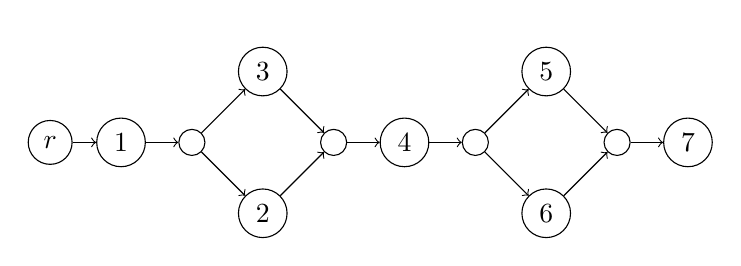
\begin{tikzpicture}[scale=0.9]
    % Nodes
    \node[draw, circle] (node1) at (0,0) {$\s{r}$};
    \node[draw, circle] (node2) at (1,0) {$\s{1}$};
    \node[draw, circle] (node3) at (2,0) {$\timesOperator$};
    \node[draw, circle] (node4) at (3,-1) {$\s{2}$};
    \node[draw, circle] (node5) at (3,1) {$\s{3}$};
    \node[draw, circle] (node6) at (4,0) {$\timesOperator$};
    \node[draw, circle] (node65) at (5,0) {$\s{4}$};
    \node[draw, circle] (node7) at (6,0) {$\plusOperator$};
    \node[draw, circle] (node8) at (7,1) {$\s{5}$};
    \node[draw, circle] (node9) at (7,-1) {$\s{6}$};
    \node[draw, circle] (node10) at (8,0) {$\plusOperator$};
    \node[draw, circle] (node11) at (9,0) {$\s{7}$};
    % Text on top
    \node[above] at (node1.north)  {$\tChartFunction$};
    \node[above] at (node2.north)  {$\tChartFunction$};
    \node[above] at (node3.north)  {                 };
    \node[above] at (node4.north)  {$\tChartFunction$};
    \node[above] at (node5.north)  {$\tChartFunction$};
    \node[above] at (node65.north) {$\tChartFunction$};
    \node[above] at (node8.north)  {$\tChartFunction$};
    \node[above] at (node9.north)  {$\tChartFunction$};
    \node[above] at (node11.north) {$\tChartFunction$};
    % Connection
    \draw[->] (node1) -- (node2);
    \draw[->] (node2) -- (node3);
    \draw[->] (node3) -- (node4);
    \draw[->] (node3) -- (node5);
    \draw[->] (node5) -- (node6);
    \draw[->] (node4) -- (node6);
    \draw[->] (node6) -- (node65);
    \draw[->] (node65) -- (node7);
    \draw[->] (node7) -- (node8);
    \draw[->] (node7) -- (node9);
    \draw[->] (node8) -- (node10);
    \draw[->] (node9) -- (node10);
    \draw[->] (node10) -- (node11);
  \end{tikzpicture}
  \caption{Pipeline Template}
  \label{fig:service_composition_template}
\end{figure}

\begin{figure}[ht!]
  \centering
  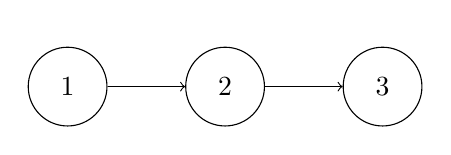
\begin{tikzpicture}
    % Nodes
    \node[draw, circle,minimum size=1cm] (node1) at (0,0) {$\s{1}$};
    \node[draw, circle,minimum size=1cm] (node2) at (2,0) {$\s{2}$};
    \node[draw, circle,minimum size=1cm] (node3) at (4,0) {$\s{3}$};

    \node[above] at (node1.north)  {$\tChartFunction$};
    \node[above] at (node2.north)  {$\tChartFunction$};
    \node[above] at (node3.north)  {$\tChartFunction$};

    % Connection
    \draw[->] (node1) -- (node2);
    \draw[->] (node2) -- (node3);

  \end{tikzpicture}
  \caption{Pipeline Template Example}
  \label{fig:temp}
\end{figure}

\subsection{Functional Transformation}\label{sec:funcannotation}

% \hl{SPIEGARE MEGLIO L'OBIETTIVO FUNZIONALE}
In order to better understand the functional aspect of the pipeline, we introduce the concept of functional transformation.
The \myGamma function is used to annotate each node with a functional transformation function \TF\ that is applied to the data.
This kind of tagging allow a more precise tracking of the data transformation throughout the pipeline.
A functions F has a twofold role:
\begin{enumerate}[label=\roman*)]
  \item it contains the functional requirements that the service must satisfy, in terms of expected input, expected output, prototype and other functional aspects.
  \item it contains the transformation function ($T$) that will be applied to the data. This function can be classified according to four types.
        \begin{enumerate*}[label=\roman*)]
          \item Function \TF{\epsilon}, an empty function that applies no transformation or processing on the data.
          \item Function \TF{a}, an additive function that expands the amount of data received, for example, by integrating data from other sources.
          \item Function \TF{t}, a transformation function that transforms some records in the dataset without altering the domain.
          \item Function \TF{d}, a transformation function that changes the domain of the data by applying, for instance, PCA or K-means (out of the scope of this work).
        \end{enumerate*}
\end{enumerate}
A transformation function can be classified according to four types.
% \begin{enumerate*}[label=\roman*)]
%   \item Function \F{e}, an empty function that applies no transformation or processing on the data.
%   \item Function \F{a}, an additive function that expands the amount of data received, for example, by integrating data from other sources.
%   \item Function \F{t}, a transformation function that transforms some records in the dataset without altering the domain.
%   \item Function \F{d}, a transformation function that changes the domain of the data by applying, for instance, PCA or K-means (out of the scope of this work).
% \end{enumerate*}

\subsection{Policy}\ref{sec:nonfuncannotation}
\hl{SPIEGARE MEGLIO L'OBIETTIVO DELLE POLITICHE}
Policies express data protection requirements, specifying access permissions based on the context and actions performed on the data.
Data protection is enforced by filtering data to return a subset, including the possibility of an empty set, rather than denying access.
We consider an attribute-based access control model that offers flexible fine-grained authorization capabilities, as the language for policy definition.
Therefore, when a user submits a resource access request, our access
control filters the returned data based on the user's privileges.
This approach ensures data protection by removing or obfuscating sensitive attributes instead of granting or denying access to the full data set.

We adapt the standard key components of an attribute-based access control model to address the unique characteristics of a big data environment.
The access control policy outlines access requirements using key components and their corresponding attributes in the following manner.

\begin{definition}[Policy Condition]\label{def:policy_cond}
  A \emph{Policy Condition} is a Boolean expression of the form $($\emph{attr\_name} op \emph{attr\_value}$)$, with op$\in$\{$<$,$>$,$=$,$\neq$,$\leq$,$\geq$\}, \emph{attr\_name} an attribute label, and \emph{attr\_value} the corresponding attribute value.
\end{definition}

A policy is then defined as follows.

\begin{definition}[Policy]\label{def:policy_rule}
  A {\it policy P} is 5-uple $<$\textit{subj}, \textit{obj}, \textit{action}, \textit{env}, \textit{\TF}$>$, where:
  \begin{description}
    \item Subject \textit{subj} defines a user or the service provider of a job issuing access requests to perform operations on objects.
          It is of the form $<$\emph{id}, \emph{PC}$>$, where \emph{id} defines a class of users (e.g., policeman), and \emph{PC} is a set of \emph{Policy Conditions} on the subject, as defined in Definition \ref{def:policy_cond}.
          For instance, $<$\emph{user},\{(role $=$ "jailer")\}$>$ refers to a person with the role of jailer.

    \item Object \textit{obj} defines any data whose access is governed by the policy.
          It is of the form $<$\emph{type}, \emph{PC}$>$, where: \emph{type} defines the type of object, such as a file (e.g., a video, text file, image, etc.), a SQL or noSQL database, a table, a column, a row, or a cell of a table, and \emph{PC} is a set of \emph{Policy Conditions} defined on the object's attributes.
          For instance, $<$\emph{dataset},\{(region $=$ CT)\}$>$ refers to a dataset whose region is Connecticut.

    \item Action \textit{action} defines any operations that can be performed within a big data environment, from traditional atomic operations on databases (e.g, CRUD operations varying depending on the data model) to coarser operations, such as an Apache Spark Direct Acyclic Graph (DAG), an Hadoop MapReduce, an analytics function call, or an analytics pipeline.

    \item Environment \textit{env} defines a set of conditions on contextual attributes, such as time of the day, location, IP address, risk level, weather condition, holiday/workday, emergency. It is a set \emph{PC} of
          \emph{Policy Conditions} as defined in Definition \ref{def:policy_cond}.
          For instance, $<$\emph{env},\{(time $=$ "night")\}$>$ refers to a policy that is applicable only at night.

    \item Data Transformation \textit{\TF} defines a set of security and privacy-aware transformations on \textit{obj}, focusing on data protection, as well as compliance to regulations and standards, in addition to simple format conversions.
  \end{description}
\end{definition}

Policies are activated upon a service's request for data access. Subsequently, policy evaluation and enforcement are executed to prepare data according to data transformation \TF\ and deliver them to the service. The core function of policy execution is to safeguard the data through operations, such as obfuscation of partial or complete records, or filter row implementation. We note that policies always permit data access, that is, policy decision is always \emph{true}. A policy decision \emph{false} applies a data transformation \TF\ such that an empty data set is returned.

\subsection{Example}\label{sec:example}
As an example, let us consider a pipeline template G(\V,\E,\myLambda,\myGamma) with three nodes, as depicted in \cref{fig:service_composition_example}.
It includes three key stages in our reference scenario: data anonymization, data enrichment, and data aggregation, each with its policy and transformation function.

\begin{enumerate*}[label=n\arabic*)]
  \item The first node is responsible for data anonymization.
        It specifies an anonymization policy ($\myLambda(v_1)$) to protect sensitive information, such as personally identifiable information (PII) in the dataset.
        The transformation function ($\myGamma(v_1)$) is an empty function, as no functional transformation is required for anonymization.
  \item The second node focuses on data enrichment, where additional information from the states of New York and New Hampshire is integrated into the dataset.
        It requires a data enrichment policy ($\myLambda(v_2)$) to ensure that the added data is relevant and compliant with privacy regulations.
        The transformation function ($\myGamma(v_2$)) is an additive function ($F_a$), which merges and integrates the external data with the existing dataset.
  \item The third node is responsible for aggregating data, including statistical measures like averages, medians, and some more statistics. It follows an aggregation policy ($\myLambda(v_3)$) to define how the aggregation should be performed and ensure compliance with privacy and security regulations.
        The transformation function (($\myGamma(v_3)$) for this node is a transformation function ($F_t$), which computes the required statistics and aggregates the data.
\end{enumerate*}

\section{Service Instance}

\begin{figure}[ht!]
  \centering
  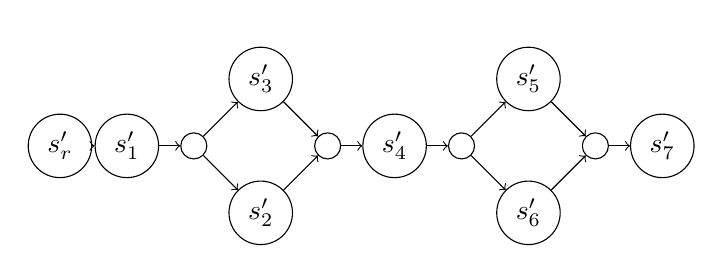
\begin{tikzpicture}[scale=0.85]
    \node[draw, circle] (node1) at (0,0) {$s^\prime_r$};
    \node[draw, circle] (node2) at (1,0) {$s^\prime_1$};
    \node[draw, circle] (node3) at (2,0) {$\timesOperator$};
    \node[draw, circle] (node4) at (3,-1) {$s^\prime_2$};
    \node[draw, circle] (node5) at (3,1) {$s^\prime_3$};
    \node[draw, circle] (node6) at (4,0) {$\timesOperator$};
    \node[draw, circle] (node65) at (5,0) {$s^\prime_4$};
    \node[draw, circle] (node7) at (6,0) {$\plusOperator$};
    \node[draw, circle] (node8) at (7,1) {$s^\prime_5$};
    \node[draw, circle] (node9) at (7,-1) {$s^\prime_6$};
    \node[draw, circle] (node10) at (8,0) {$\plusOperator$};
    \node[draw, circle] (node11) at (9,0) {$s^\prime_7$};
    % Text on top
    \node[above] at (node1.north) { \footnotesize$\iChartFunction$};
    \node[above] at (node2.north) { \footnotesize$\iChartFunction$};
    \node[above] at (node3.north) {};
    \node[above] at (node4.north) { \footnotesize$\iChartFunction$};
    \node[above] at (node5.north) { \footnotesize$\iChartFunction$};
    \node[above] at (node65.north) { \footnotesize$\iChartFunction$};
    \node[above] at (node8.north) { \footnotesize$\iChartFunction$};
    \node[above] at (node9.north) { \footnotesize$\iChartFunction$};
    \node[above] at (node11.north) { \footnotesize$\iChartFunction$};
    % Connection
    \draw[->] (node1) -- (node2);
    \draw[->] (node2) -- (node3);
    \draw[->] (node3) -- (node4);
    \draw[->] (node3) -- (node5);
    \draw[->] (node5) -- (node6);
    \draw[->] (node4) -- (node6);
    \draw[->] (node6) -- (node65);
    \draw[->] (node65) -- (node7);
    \draw[->] (node7) -- (node8);
    \draw[->] (node7) -- (node9);
    \draw[->] (node8) -- (node10);
    \draw[->] (node9) -- (node10);
    \draw[->] (node10) -- (node11);
  \end{tikzpicture}
  \caption{Service composition instance}
  \label{fig:service_composition_instance}
\end{figure}

\subsection{Instance}
\hl{ANCHE QUA COME PER IL TEMPLATE PROVEREI A ESSERE UN POCO PIU' FORMALE. GUARDA IL PAPER CHE TI HO PASSATO.} When the template is filled with the necessary services, it becomes an instance that reflects the actual implementation of those services.
This instance follows the same flow as the template, but but both \myLambda and \myGamma are replaced respectively by \iChartFunction~ which represent the transformation operations carried out by the service.

\begin{definition}[Pipeline Instance]\label{def:instance}
  Let \G(\V,\E,\myLambda,\myGamma) be a Service Template, a Service Instance \G'(\V',\E,$\iChartFunction$) is a directed acyclic graph where:
  \emph{i)} $s_r$$=$$s'_r$, \emph{ii)} for each vertex \vi{}$\in$\V$_{\timesOperator}$$\cup$\V$_{\plusOperator}$ it exists a corresponding vertex \vii{}$\in$\Vp$_{\timesOperator}$$\cup$\Vp$_{\plusOperator}$,
      and for each \vi{i}$\in$\V$_S$ annotated with policy \Pset{i} it exists a corresponding \vii{i}$\in$ \Vp$_S$ instantiated with a real service $s_i$, such that the following conditions hold:
  \begin{itemize}
    \item $s_i$ satisfies functional requirements in \G(\Vp,\E,\iChartFunction).
    \item \Pset{i} satisfies $\iChartFunction(v_i)$.\hl{QUESTA SECONDA NON MI TORNA}
  \end{itemize}
\end{definition}

\hl{SPIEGHIAMO IL SIGNIFICATO DELLE CONDIZIONI, MENZIONANDO ANCHE IL RUOLO DI}\F{}\hl{ NELLA CONDIZIONE 1.}

The Service  Instance  is generated by traversing the Service Template with a breadth-first search algorithm, starting from the root vertex \vi{r}. Then for each vertex \vi{i} in the pipeline template, the corresponding vertex \vii{i}$\in$\Vp\ is generated. Finally, for each vertex \vii{i}$\in$\Vp, a two-step selection approach is applied as follows.
\begin{itemize}
  \item \textit{Filtering Algorithm} - It matches requirements in $\iChartFunction$ with the policy $\iChartFunction$, and returns a set of services $S_i$ that satisfy the requirements.\hl{NON CHIARA}
  \item \textit{Comparison Algorithm} - Upon retrieving a set of compatible services, it produces a ranking of these services according their scoring function. The scoring function is calculated according some metrics, which evaluate the quality of the data resulting from the service execution. More details about the metrics are provided in Section \ref{sec:metrics}.\hl{ANCHE QUESTA PUO ESSERE MODIFICATA, VEDERE ALTRO PAPER.}
\end{itemize}

\hl{METTIAMO UNA CHIOSA CHE DICE CHE DOPO IL COMPARISON ABBIAMO UN'ISTANZA COMPLETA}

\begin{example}
  \hl{TODO}
\end{example}


% \begin{figure}[H]
%   \centering

%   \begin{tikzpicture}
%     % Nodes
%     \node[draw, circle, minimum size=0.4cm, draw=gray, text opacity=0.5] (node11) at (0,1.2) {Sx};
%     \node[draw, circle, minimum size=1cm] (node1) at (0,0) {S1};
%     \node[draw, circle, minimum size=0.4cm, draw=gray, text opacity=0.5] (node10) at (0,-1.2) {Sy};

%     \node[draw, circle, minimum size=0.4cm, draw=gray, text opacity=0.5] (node22) at (2,1.2) {Sx};
%     \node[draw, circle, minimum size=1cm] (node2) at (2,0) {S2};
%     \node[draw, circle, minimum size=0.4cm, draw=gray, text opacity=0.5] (node21) at (2,-1.2) {Sy};

%     \node[draw, circle, minimum size=1cm] (node3) at (4,0) {$\timesOperator$};

%     \node[draw, circle, minimum size=0.4cm, draw=gray, text opacity=0.5] (node42) at (5,-1.5) {Sx};
%     \node[draw, circle, minimum size=1cm] (node4) at (6,-1.5) {S3};
%     \node[draw, circle, minimum size=0.4cm, draw=gray, text opacity=0.5] (node41) at (7,-1.5) {Sy};

%     \node[draw, circle, minimum size=1cm] (node5) at (6,1.5) {S4};
%     \node[draw, circle, minimum size=0.4cm, draw=gray, text opacity=0.5] (node51) at (5,1.5) {Sx};
%     \node[draw, circle, minimum size=0.4cm, draw=gray, text opacity=0.5] (node52) at (7,1.5) {Sy};
%     % Connection
%     \draw[->] (node1) -- (node2);
%     \draw[->] (node2) -- (node3);
%     \draw[->] (node3) -- (node4);
%     \draw[->] (node3) -- (node5);
%   \end{tikzpicture}
%   \caption{Service composition instance}
%   \label{fig:service_composition_instance}
% \end{figure}
% \[ \forall S \in \mathrm{S}_{C}  \exists  \iChartFunction(S) = \mathrm{S}_{1} \]


\begin{figure}
  \centering
  \includegraphics[width=\columnwidth]{serviceDetail.pdf}
  \caption{Service Detail}
  \label{fig:service_detail}reinstall remote-ssh
\end{figure}
